\chapter{The dataset}\label{cha:data}

This chapter introduces the dataset and work done to enable information extraction and analysis of the provided data. The case for the analysis is also introduced.


% In the data set, three power plants have Pelton turbines with measurement of their needle position. More information about a Pelton turbine can be found in chapter \ref{cha:data}. One of the power plants had recorded several issues with the control and behavior of the needles during operation. There were many interesting events spread out over many of the power plants, but one major benefit with the Pelton needle case was that there was one plant with several reported issues for the same component. In most of the other cases, there were only recorded one incident on one plant, making them hard to analyze and validate. The fact that there are two additional power plants with the same process signals without reported issues opened up the possibility for testing and validating the chosen techniques not only on data from the faulty plant. This also introduced the possibility to validate how well and how easy the different techniques could adapt to new plants.    




% Based on the arguments above, the Pelton needle case was chosen as the focus of the thesis. The following points were then defined as a basis for the analysis. 


\section{Dataset}\label{sec:dataset}
    Hymatek controls provided a dataset from a Norwegian energy company, containing process information from $27$ hydroelectric powerplants logged from $2013$ to mid $2017$. The data is not pre-processed in any way, and come just as it is logged at the company. A big part of the thesis has been spent on exploring the data, finding out what is logged and what can be used. The data is split into five folders, one for each year. In each folder, several different files are stored. Table \ref{tab:data_files} shows the different file types that are found in the dataset. The file names indicated the frequency, sampling type and sampling duration of the data. The files are not separated by plants, only by date. Hence, a file containing data sampled every second for any given start and stop date contains data from all plants for that given period. In addition to the data files, a meta-data file is provided where plant name and process signal for each tag can be found.
    
    \begin{table}[]
        \centering
        \begin{tabular}{c c c c c}
        
        \toprule
             \textbf{Interval}   & \textbf{Average}   & \textbf{Max}   & \textbf{Min}   & \textbf{Actual}    \\ \midrule
             Daily      & x         & x     & x     & -         \\ 
             Hourly     & x         & x     & x     & -         \\ 
             Minutely   & x         & x     & x     & -         \\ 
             Secondly   & -         & -     & -     & x         \\ \bottomrule
        \end{tabular}
        \caption{Table showing the available data for the different sampling frequencies}
        \label{tab:data_files}
    \end{table}
    
    The total size of all files exceeded $90$Gb. This means that one can't merely load all data into the computer memory, and work with it from there. The information needs to be extracted one plant at a time, for each of the different sampling rates and stored in a way that enabled fast and efficient loading.

    
    \subsection{Old and new data format}\label{subsec:data_format}
        Regardless of sampling-rate and data type, the files are all in the same format. As seen in Table \ref{tab:orig_data}, each line holds a tag, a time of sampling and process value. 
        \begin{table}[h]
            \centering
            \begin{tabular}{c c c}
                \toprule
                 \textbf{Tag}        & \textbf{Timestamp}         & \textbf{Value}  \\ \midrule
                 192390514  & 20170101000000000 & 0.897244155 \\
                 192391514  & 20170101000000000 & -0.549806237 \\ \bottomrule
            \end{tabular}
            \caption{Example of the structure of the original datasets}
            \label{tab:orig_data}
        \end{table}
        Once a file is loaded the tag is replaced by the process-signal name found in the meta-data file. To enable interpretation and analysis of the data, it is decided that new datasets needs to be created on the format shown in Table \ref{tab:plant_format}.
        \begin{table}[h]
            \centering
            \begin{tabular}{c c c c c }
                \toprule
                \textbf{Time stamp} & \textbf{P. variable 1}     & \textbf{P. variable 2}    & \textbf{..}    & \textbf{P. variable n}    \\ \midrule
                time 1        & NaN         & $2$           & ..    & NaN         \\ 
                time 2        & $3.00$      & NaN           & ..    & $0.00214$\\ 
                :            & :            & :             & ..    & : \\ 
                time n        & $1.00$      & NaN           & ..    & $0.814$\\ \bottomrule
            \end{tabular}
            \caption{Example showing how the data looks for each plant after reconstruction is complete}
            \label{tab:plant_format}
        \end{table}

        
    \subsection{Overview of the datasets}
        Once the data is reconstructed as specified in subsection \ref{subsec:data_format} one can look into what information it holds. The number of available process signals varies a lot, from above $250$ to below $20$, as can be seen in Figure \ref{fig:process_signal_overview}. This is used as a first stage filtering to reduce the number of plants to examine. The plants with fewer than $30$ process-signals are dropped from the analysis, reducing the number of plants in the dataset to $15$.    
        
        \begin{figure}[h]
            \centering
            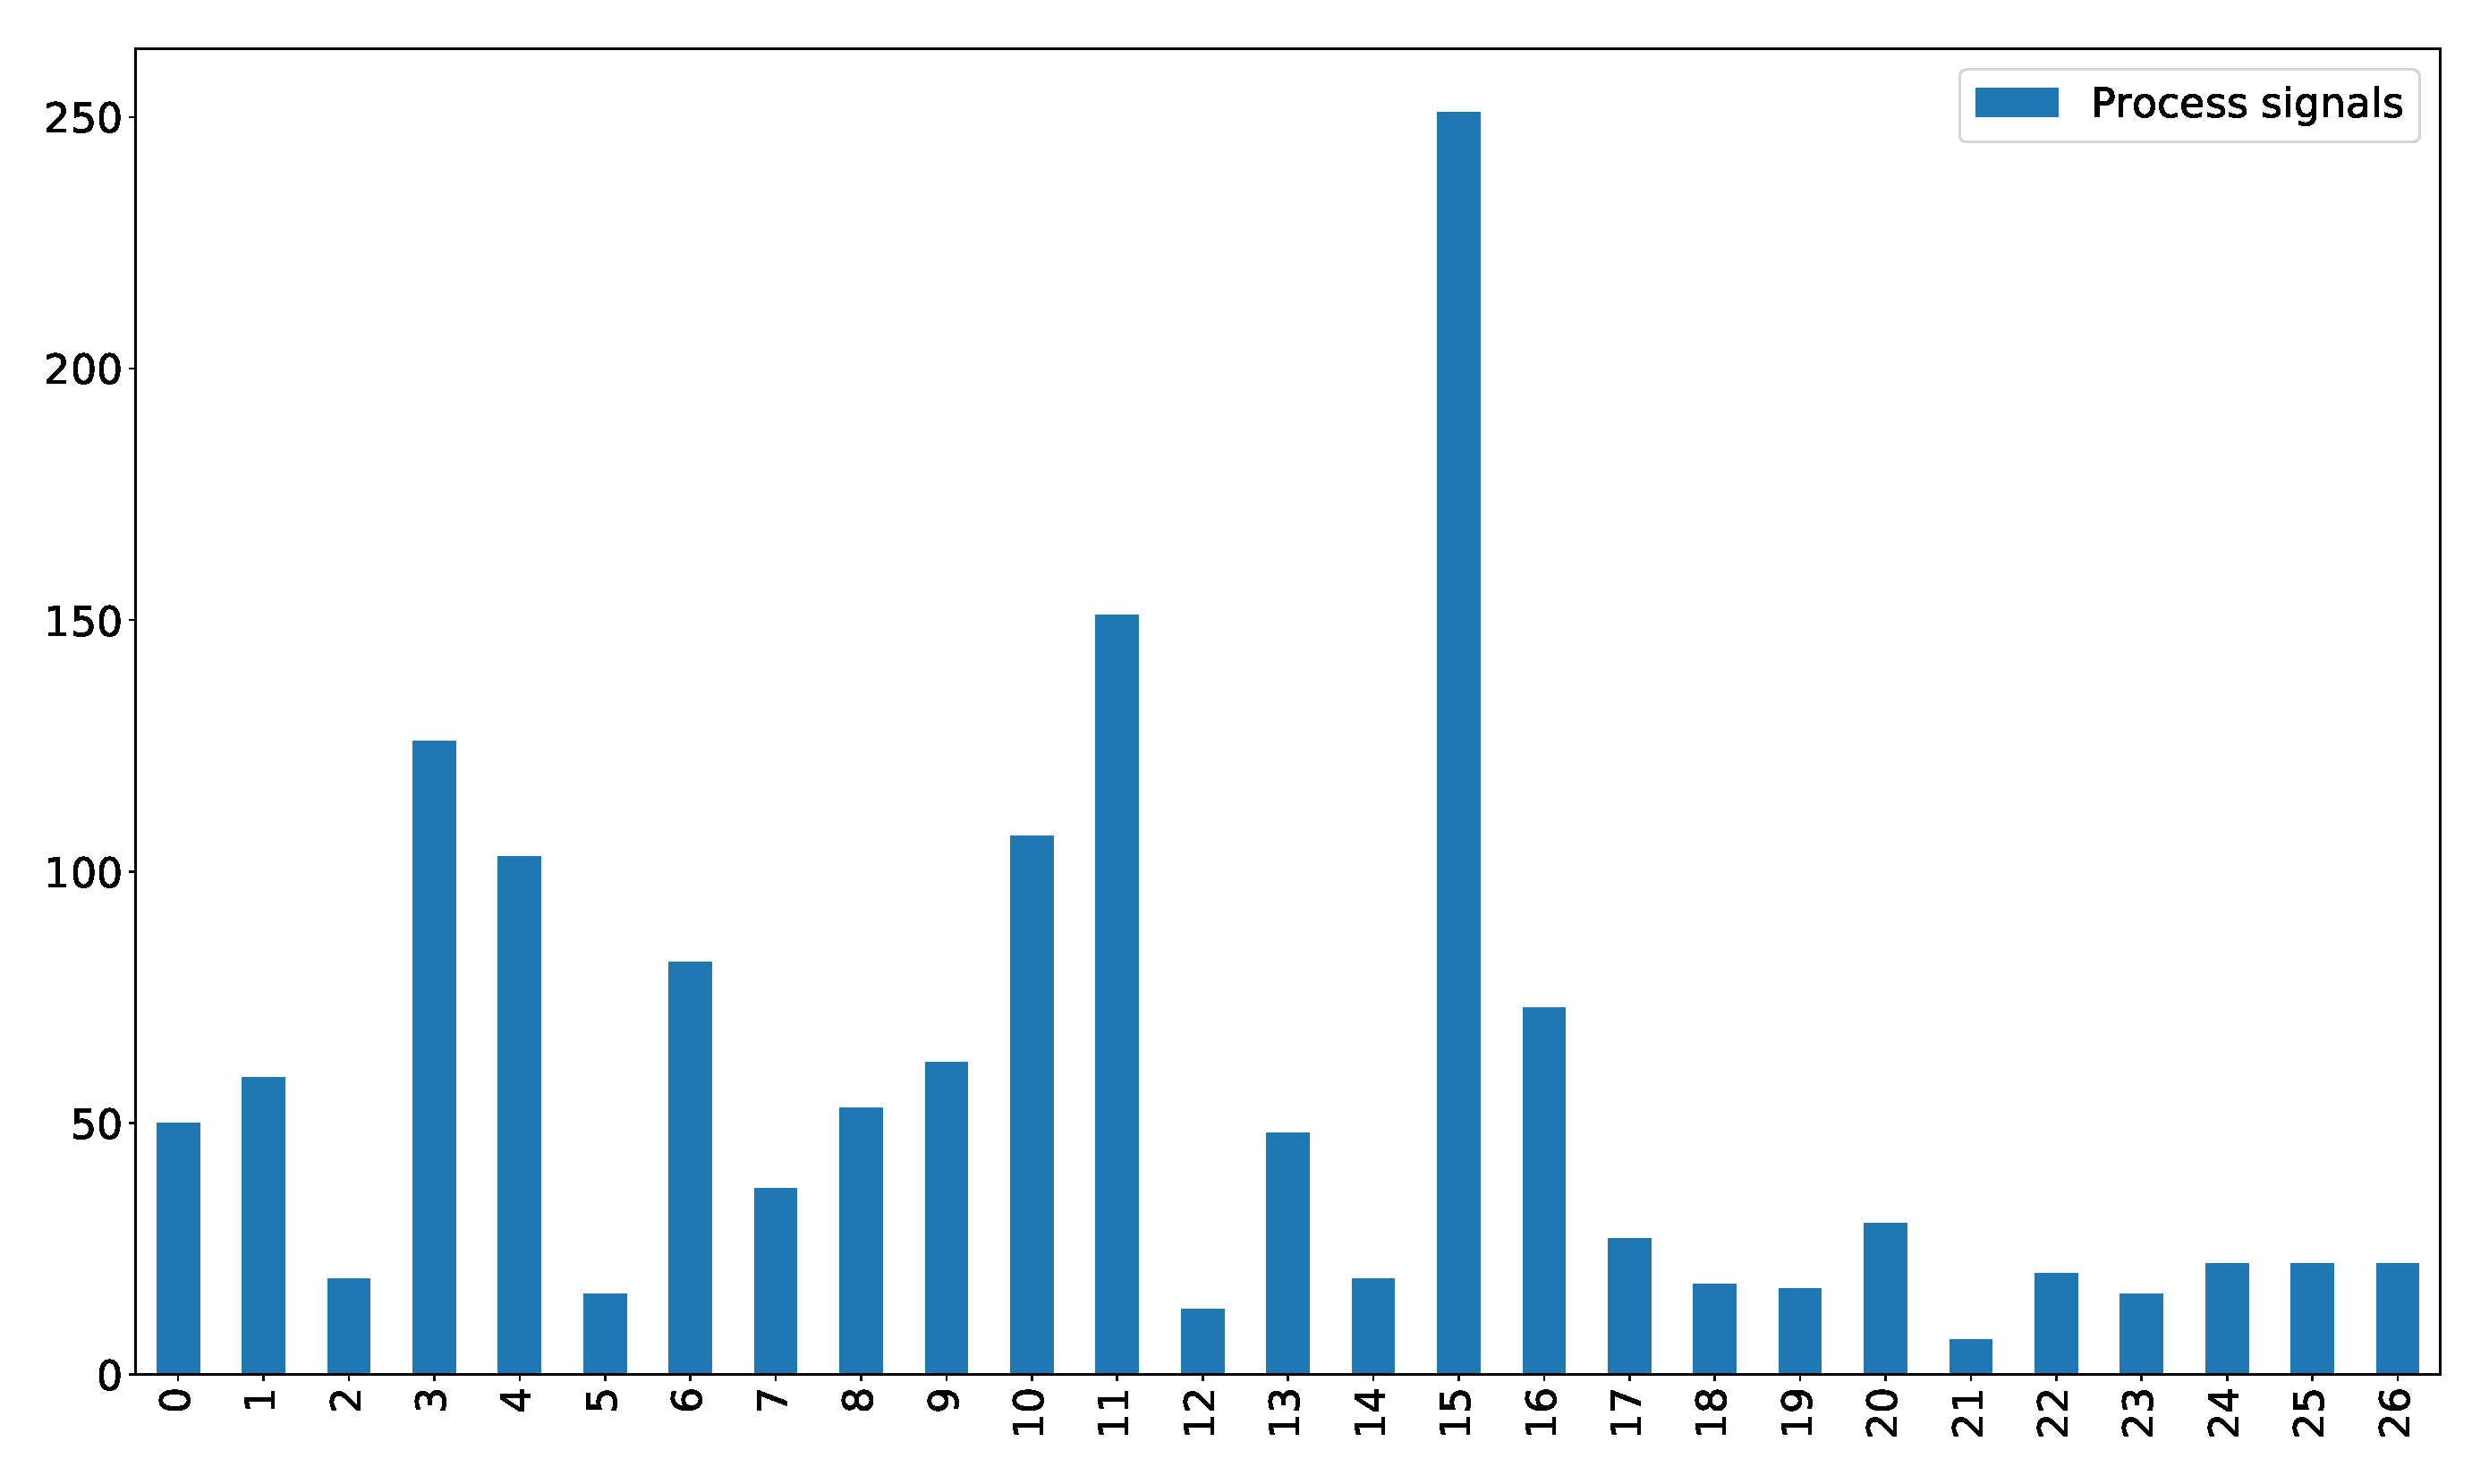
\includegraphics[width=\textwidth]{report/figures/data/plant_process_signals_overview.pdf}
            \caption{Overview of the number of process-signals or features for each of the 27 plants in the dataset.}
            \label{fig:process_signal_overview}
        \end{figure}
        
        After discarding the plants with few signals, the type of process-signals available is looked into. The more data sampled from different parts of a plant, the better. Having data from several parts and components of a plant can enable finding a link between unknown components and sensors. Figure \ref{fig:signal_type_overview} shows the different types of signals found in the datasets for the different plants. As can be seen, the temperature is one of the most common signals for all plants. There is also many signals of type "Def Type Måling", which is a common name that covers all signals not defined with a unique tag. Pressure, level, vibration, and so on are signals covered by this tag. Since all of the remaining plants had process-variables of different types, none are removed. 
        
        \begin{figure}
            \centering
            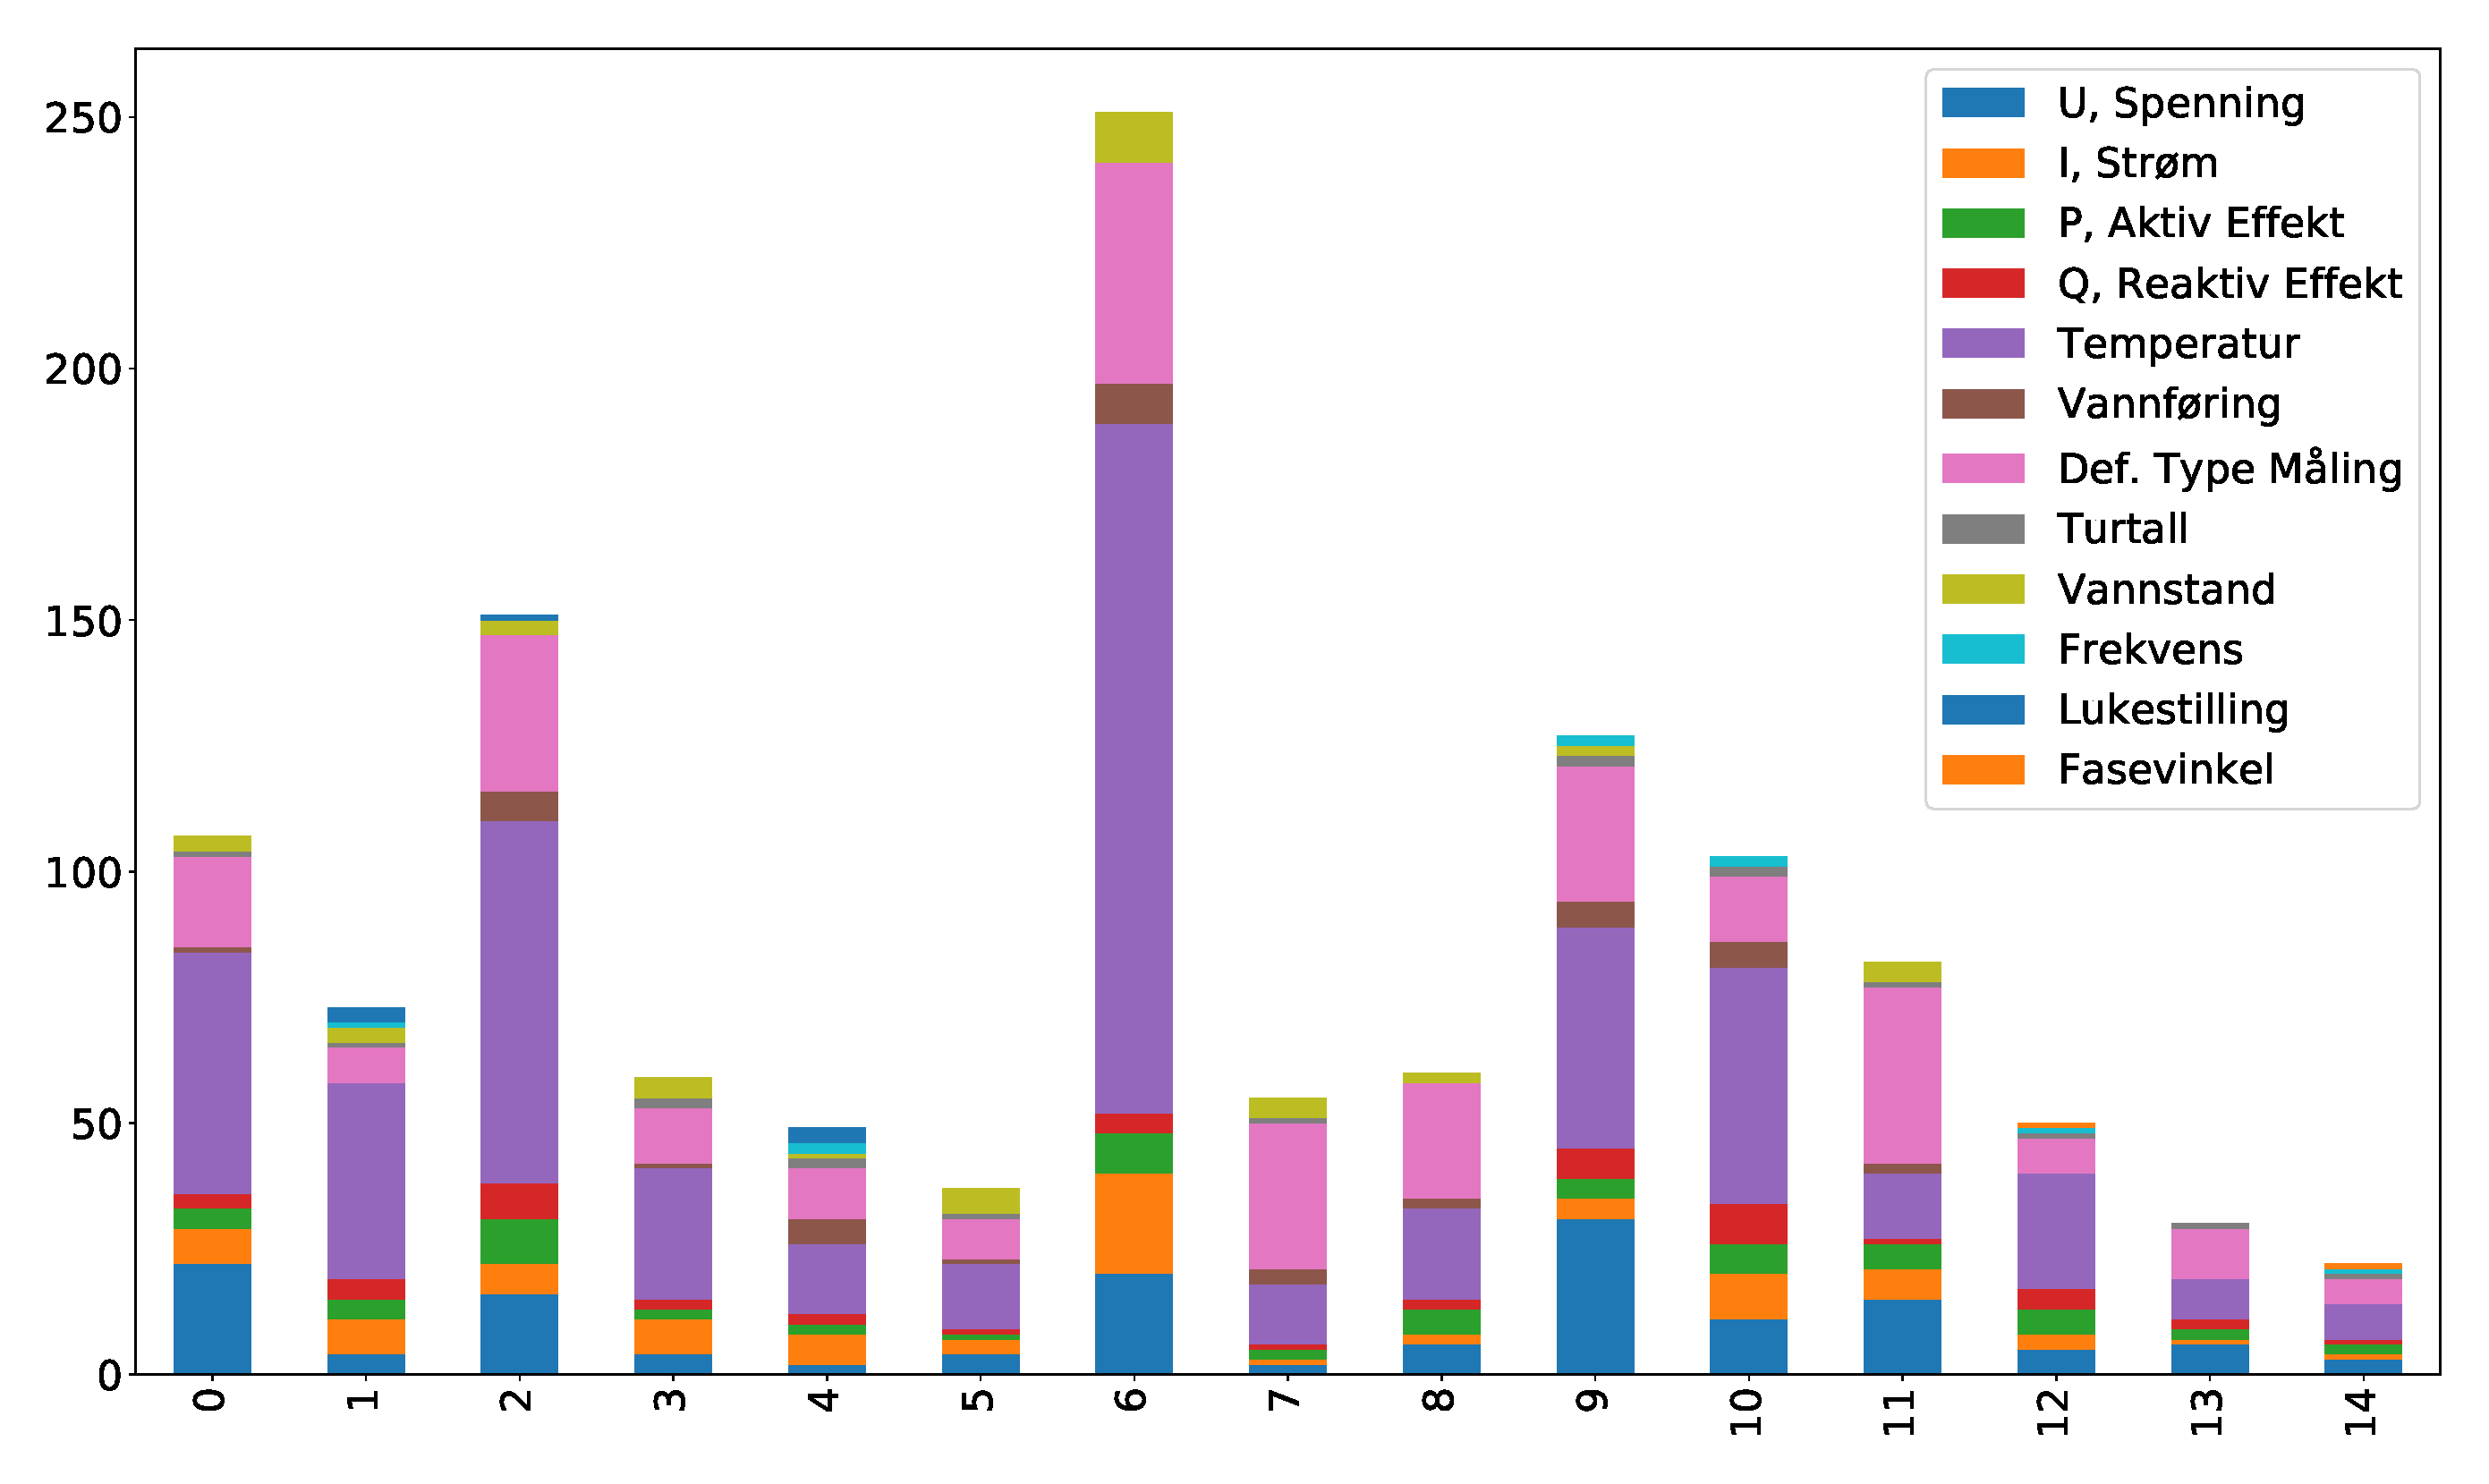
\includegraphics[width=\textwidth]{report/figures/data/plant_signal_types_overview.pdf}
            \caption{Figure showing the different process signals or features found at each of the 27 plants in the dataset.}
            \label{fig:signal_type_overview}
        \end{figure}
        
        % It is only necessary to keep the datasets with the highest sampling rate. The highest sampling rate will provide the most detail about a plant, and lower sampling rates can always be extracted from higher rates.
        
        % was decided to only use the datasets sampled every second. Using these datasets gave a snapshot of the plant state at a given time. Pandas have a lot of built-in functionality that enables easy re-sampling so that the average, max and min datasets could easily be recreated from this dataset if wanted.
        
        An issue arose when looking in detail at the datasets. Preferably, all process-signals should be sampled periodically and at the same time. This is however not the case, only at hourly resolution are the data matrices complete. At higher sampling rates there are a lot of missing data. At the highest sampling frequency (every second), there are many time-stamps where none of the process signals are sampled, and those that are sampled, often only samples one process-signal. This means that one either has to work with only hourly sample rate, work with incomplete datasets or reduce the number of process signals to investigate. Either the equipment used for sampling is not working as it should, or the varying sampling rate must be on purpose. It could be that a similar sampling scheme to the one seen in \cite{Selak2014} is used. This is however not possible to confirm from the data alone, and the energy company did not provide this information. This sheds light on the fact that having lots of data is not always a sign of quality. The data sampled in $2013$ is poorer than the later years, and hence it is dropped from any further analysis. 
    % \subsection{Instrumentation}\label{subsec:instrumentation}
    %     what is there of instrumentation? refer to the data I have gotten         
        
    \subsection{The historical log of the plants }
        Once an overview of the data was in place, the energy company was contacted, requesting an incident log from the remaining plants. Incident logs for the entire sampling period, for all of the $27$ power plants, were received. The level of details in the logged incidents is very varying from plant to plant. Some plants have reported over 200 incidents, while others barely exceeded 20. Many of the incidents are also minor incidents like a broken light bulb or nonfunctioning tools. Finding interesting incidents was time-consuming. Several interesting incidents were found, but very few were reported to occur more than once. Having few incidents makes it hard to separate valuable information from noise. Only having a limited number of faults can easily lead to overfitting. There is always a risk that randomness can cause the correlations and variable dependencies found. This needs to be taken into consideration when working such cases.  
        
        In the log for one of the power plants, it was found an error with the needles for a Pelton turbine. The error reported that as the opening of needle four of turbine two decreased below $46\%$, it started to lag behind needle two. The plant has two turbines that both have four needles. A search through the $14$ remaining power plants showed that there are two additional plants with Pelton turbines. One with four needles and one with five. These plants have however not reported any problems with the Pelton needles. This could then be a possible reference for normal operation. Also, it opens the possibility for testing how adaptable the anomaly detection methods are. 
        
        % \todo{remove this or add more analysis}When looking into the historical log of the plant, it was found that several more incidents with the Pelton needles were reported for the two turbines
        
\section{Pelton needles case}\label{sec:pelton_needles}
    The Pelton needle case was chosen for further analysis for several reasons. Firstly it is a critical part of the Pelton turbine if the needles are not operating as they should it will affect the power produced by the turbine. The needle openings are a big part of a complex control system, that controls that the turbine holds a constant speed. Finding a method that can give early warnings about incidents like the one above, means maintenance can be planned, and components overhauled before the system condition becomes too severe. Secondly, having data from different plants makes it possible to analyze how well the methods and techniques used to adapt to new data. This is an important factor, if one can develop a method that is transferable with little to no adaptation need between plants, the time for commissioning will be significantly reduced. In addition, this case fits well as an extension of \cite{Aasnes2017}, where the condition of the guide vanes for a Francis turbine was analyzed. Finally, quality and available process variables vary a lot from plant to plant. One of the most significant issues was that the majority of the process signals were not sampled at a constant frequency. The Pelton needles were found to be sampled in a manner that allowed the use of data from two separate plants.
             

    \subsection{Pelton needle incident 02.03.2017}
        As the incident reported that one needle was lagging behind another, it could indicate pairwise operated needles. This can also be justified from a practical perspective if the needles are placed opposite of each other they will give the turbine an even momentum as long as they lead the same amount of water onto the turbine. To confirm this, scatter-plots were created where each needle is plotted against the other. To enable this the needle process signals are pairwise extracted from the rest of the dataset, and all time-stamps where both needles are not sampled are removed. Figure \ref{fig:plant1_needles} shows the scatter-plot of the pairwise operated needles for both turbines at plant 1. As can be seen in all four plots, the majority of the data follows a linear dependency between the needles. However, several data-points deviate from this, especially for needle pair $[2,4]$ on turbine $2$, which had the reported incident. The plot in the bottom right corner shows what appears to be operational problems. It is only needle [1,3] on turbine one seen in the upper left plot, which follows the linear pattern.
        \begin{figure}
            \begin{minipage}[b]{0.5\linewidth}
                \centering
                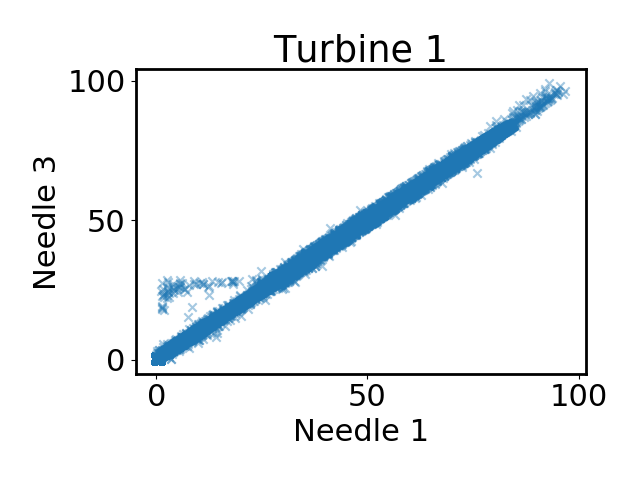
\includegraphics[width=\textwidth]{report/figures/data/t1_n1_n3.png}
            \end{minipage}
            \begin{minipage}[b]{0.5\linewidth}
                \centering
                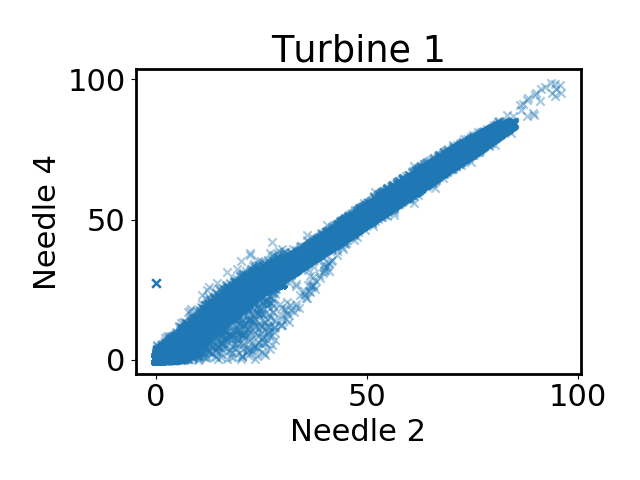
\includegraphics[width=\textwidth]{report/figures/data/t1_n2_n4.png}
            \end{minipage}
            \begin{minipage}[b]{0.5\linewidth}
                \centering
                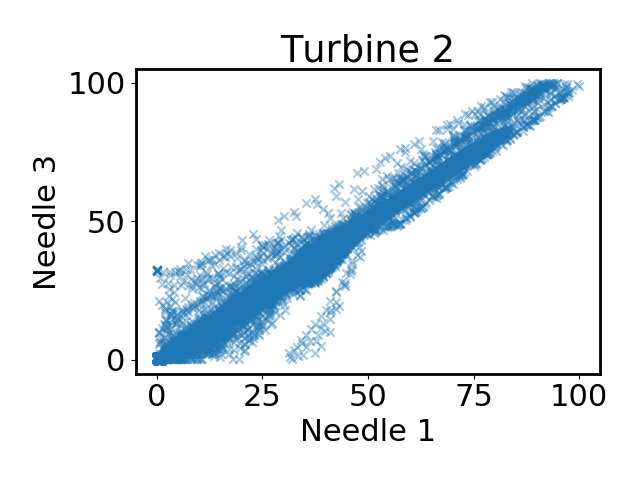
\includegraphics[width=\textwidth]{report/figures/data/t2_n1_n3.png}
            \end{minipage}
            \begin{minipage}[b]{0.5\linewidth}
                \centering
                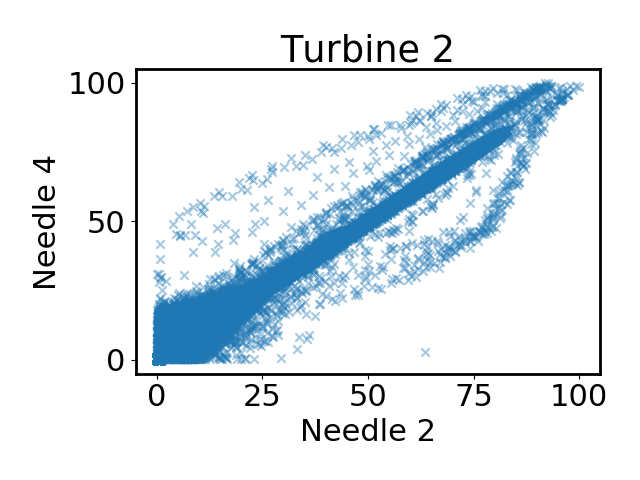
\includegraphics[width=\textwidth]{report/figures/data/t2_n2_n4.png}
            \end{minipage}
            \caption{Needle openings for the pairwise operated needles for both turbines at Plant 1 are scatterplotted in four sub-figures.}
            \label{fig:plant1_needles}
        \end{figure}
        
        % \begin{figure}[h]
        %     \centering
        %     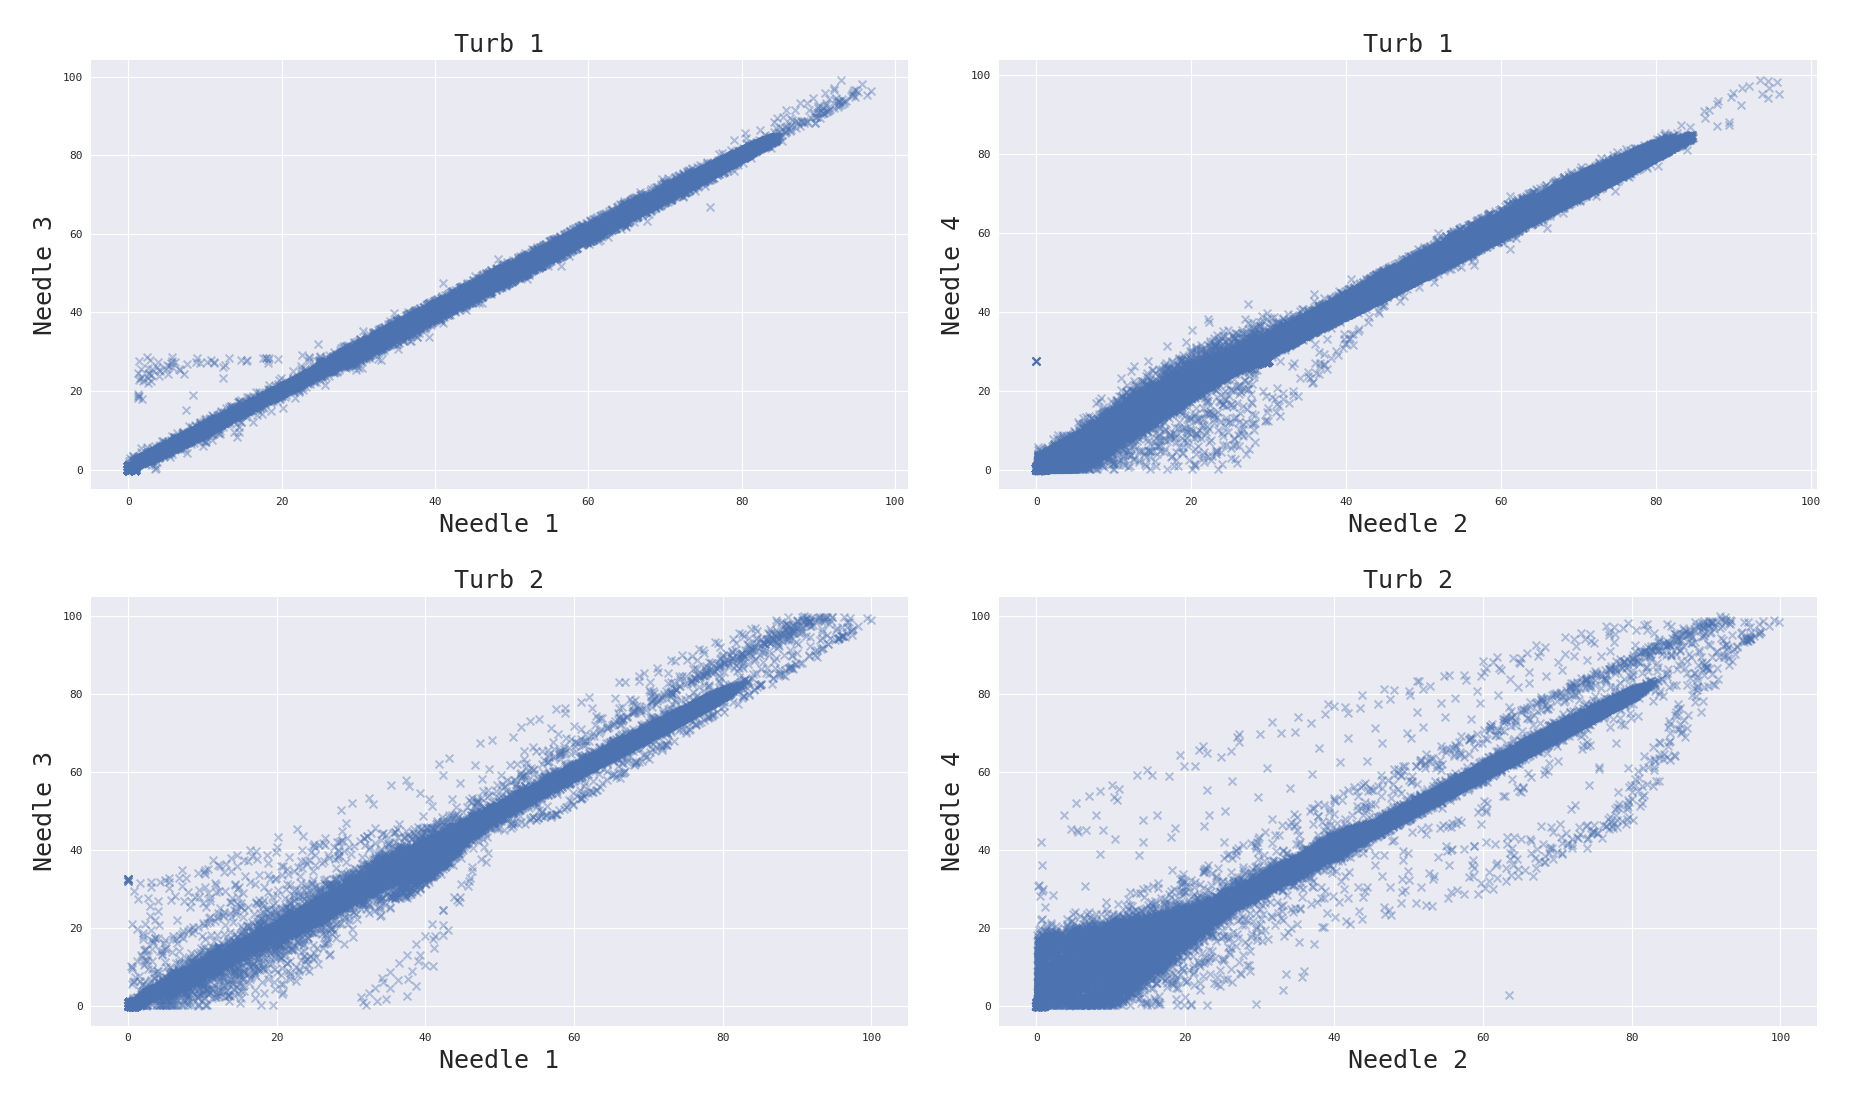
\includegraphics[width=\textwidth]{report/figures/data/plant1_needles.png}
        %     \caption{Pairwise operated needles for the two turbines at Plant 1 are scatterplotted in four subfigures. }
        %     \label{fig:plant1_needles}
        % \end{figure}
        % Figure \ref{fig:n_pos_0203} to \ref{fig:n_pos_aft_0303} shows the needle positions for two dates surrounding the reported incident, and all data after. Figure \ref{fig:n_pos_aft_0303} show that the problem was fixed when reported in early March. Figure \ref{fig:n_pos_0203} and \ref{fig:n_pos_0303} shows the two days with worst performance, and one can see that many of the worst data-points from the lower right plot in figure \ref{fig:plant1_needles}, looks to be the same as the ones shown in figure \ref{fig:n_pos_0203} and \ref{fig:n_pos_0303}.
        \begin{figure}
            \centering
            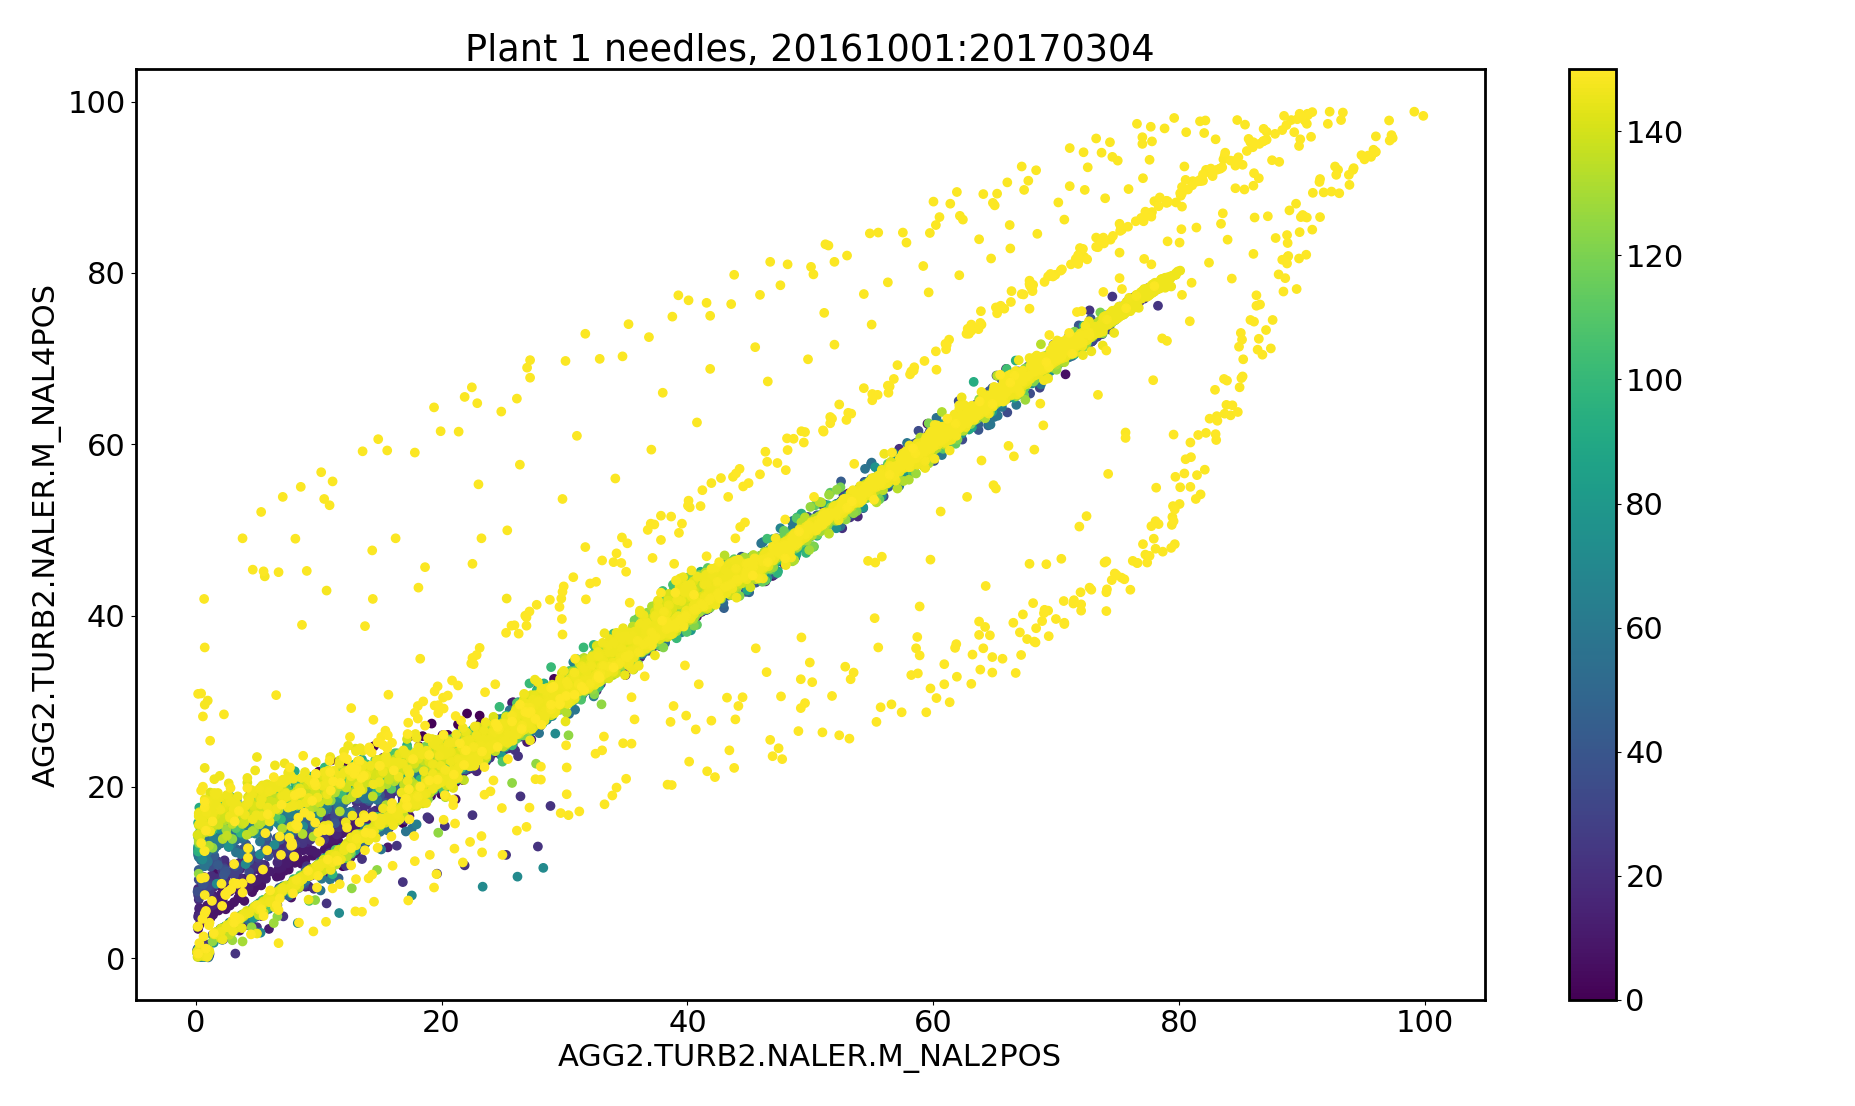
\includegraphics[width=\textwidth]{report/figures/analysis/plant1_error/needle_2_4_20161001-20170304_dots.png}
            \caption{Scatterplot of needle 2 and 4 at Plant 1 turbine 2 of the 150 days leading up to the incident. The color of a sample indicates when it is sampled. The color bar to the right shows how the color change with time. Day 0 is 150 days before the incident. The opening of needle 2 is along the x-axis, and the opening of needle 4 is along the y-axis.}
            \label{fig:plan1_scatter_20161001-20170304}
        \end{figure}
        Figure \ref{fig:plan1_scatter_20161001-20170304} shows a scatter plot of the needles [2,4] for the last 150 days up to the reported incident. The sample color changes as days go by, as seen in the color bar. It becomes clear that the most deviating samples are from the days around the incident. There are very few dark samples that deviate from the linear pattern, indicating normal system operation 150 days before the incident. Figure \ref{fig:plan1_scatter_20161001-20170304_40} shows the same plot zoomed in. Looking at the bottom left corner of the plot, one can see that needle 4 is lagging behind needle 2. It is also clear that the lag is worsening with time, as the color is shifting from dark to yellow. What happens the day of the incident is hard to explain, and the data takes on a completely new pattern. Unfortunately, it was not possible to get the full information from the energy company about what maintenance was performed to fix this problem. It is therefore assumed that the incident is a result of the system degradation seen leading up to 02.03.2017 and that this pattern can be used to detect similar system degradation before the performance becomes unacceptable.     
        \begin{figure}
            \centering
            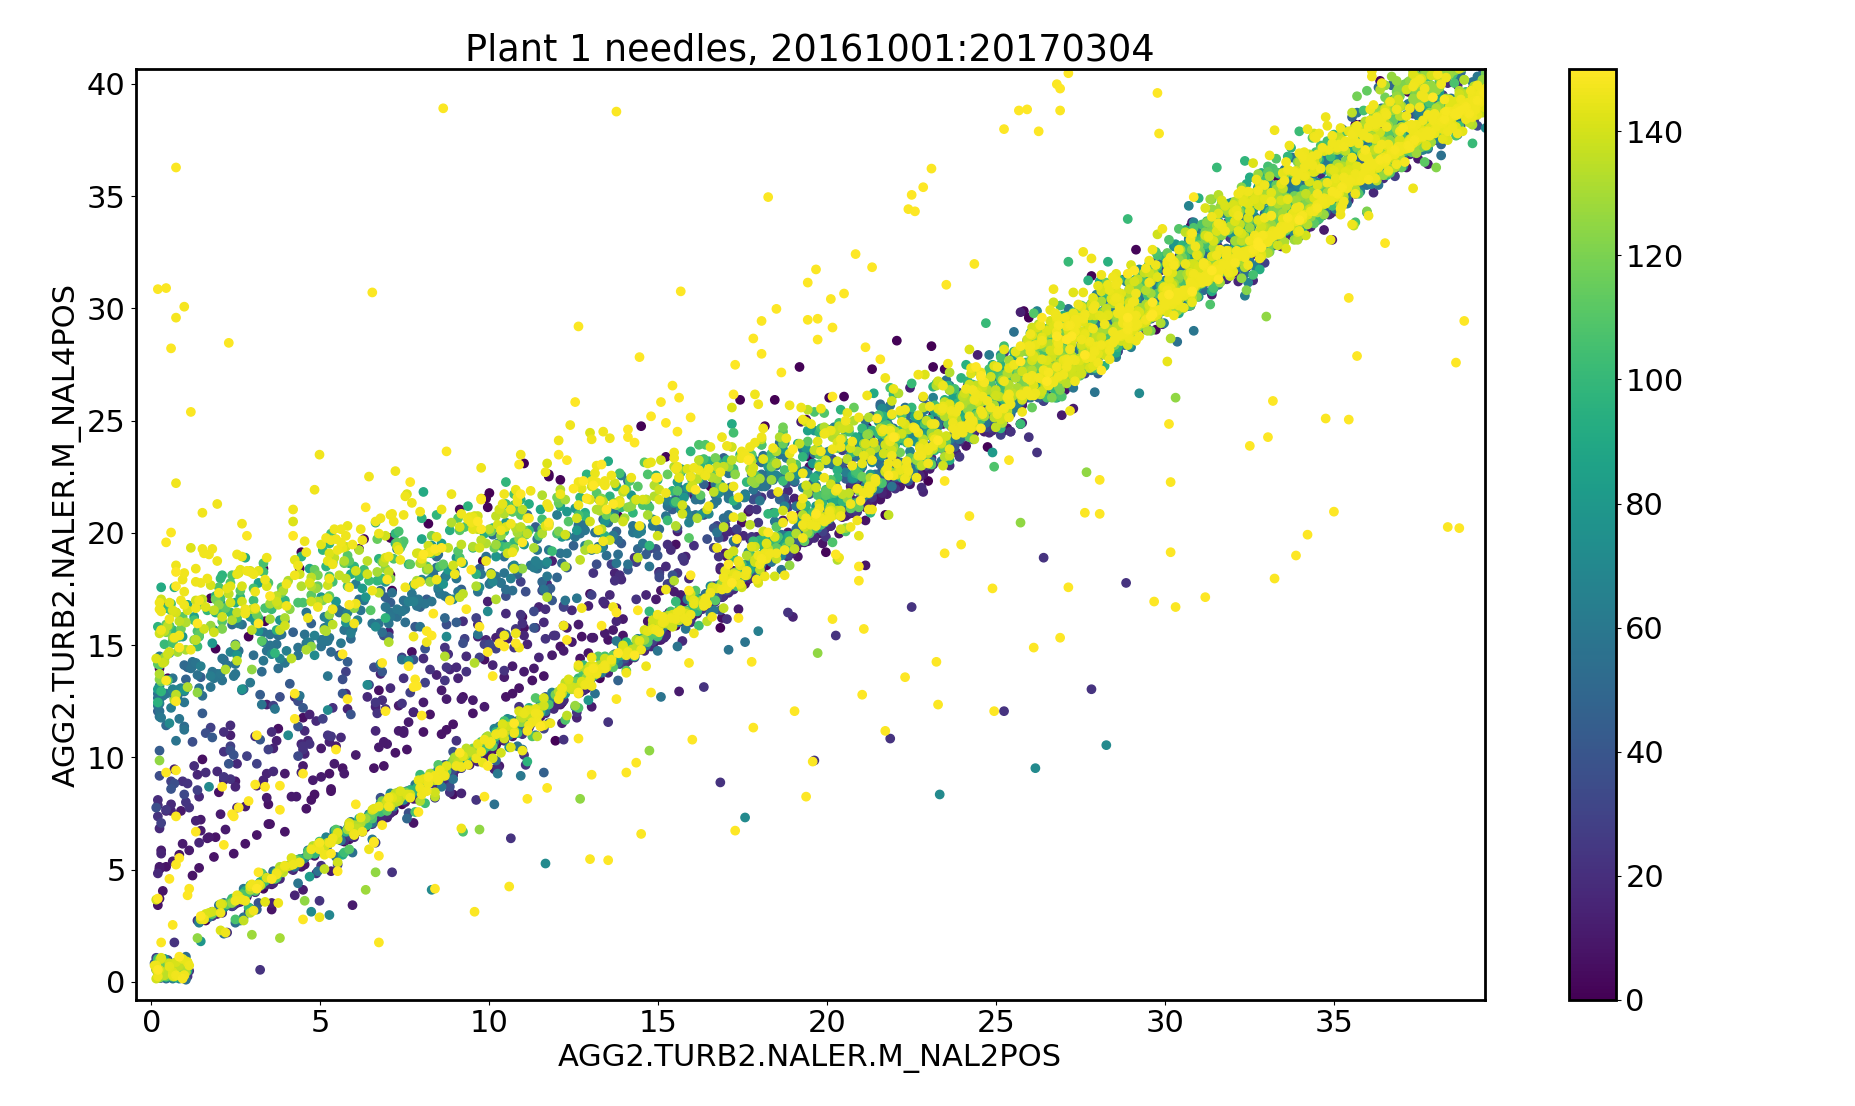
\includegraphics[width=\textwidth]{report/figures/analysis/plant1_error/needle_2_4_20161001-20170304_40_dots.png}
            \caption{Turbine 2 needle [2,4] scatterplot of the 150 days leading up to the incident zoomed in. How to interpret the figure can be seen in Figure \ref{fig:plan1_scatter_20161001-20170304}.}
            \label{fig:plan1_scatter_20161001-20170304_40}
        \end{figure}
        
        % \begin{figure}[h!]
        %     \caption*{Turbine 2 needle positions}
        %     \begin{minipage}[b]{0.5\linewidth}
        %         \centering
        %         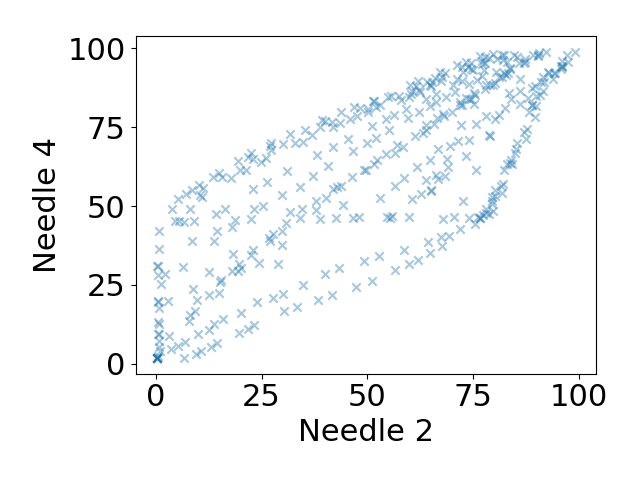
\includegraphics[width = \textwidth]{report/figures/data/turb2_n2_n4_02032017.png}
        %         \caption{02.03.2017}
        %         \label{fig:n_pos_0203}
        %     \end{minipage}
        %     \begin{minipage}[b]{0.5\linewidth}
        %         \centering
        %         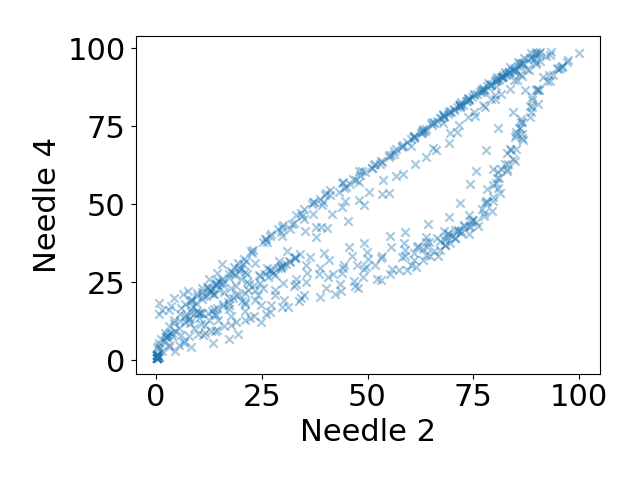
\includegraphics[width = \textwidth]{report/figures/data/turb2_n2_n4_03032017.png}
        %         \caption{03.03.2017}
        %         \label{fig:n_pos_0303}
        %     \end{minipage}
        %     \begin{minipage}[b]{0.5\linewidth}
        %         \centering
        %         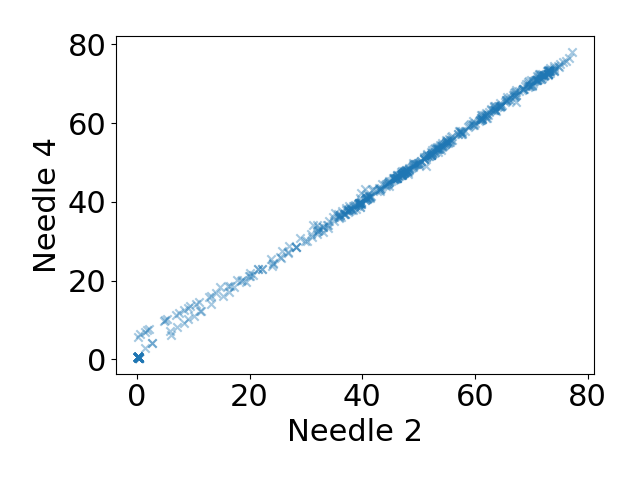
\includegraphics[width = \textwidth]{report/figures/data/turb2_n2_n4_after_04032017.png}
        %         \caption{04.03.2017 ->}
        %         \label{fig:n_pos_aft_0303}
        %     \end{minipage}
        % \end{figure}
        
        To investigate how the turbine had performed earlier in the sampling period, Figure \ref{fig:plant1_needle_error} was created. It shows the needles positions on top of each other, and the error between them. The reported incident $02.03.2017$ can be seen in the plot. The claim made earlier that the system is gradually degrading can be supported by the growing error up to the incident. Interestingly, there also seem to have been some issues with the operation in both 2014 and 2016. There is, however, no reported incidents in the plant log. 
        \begin{figure}
            \centering
            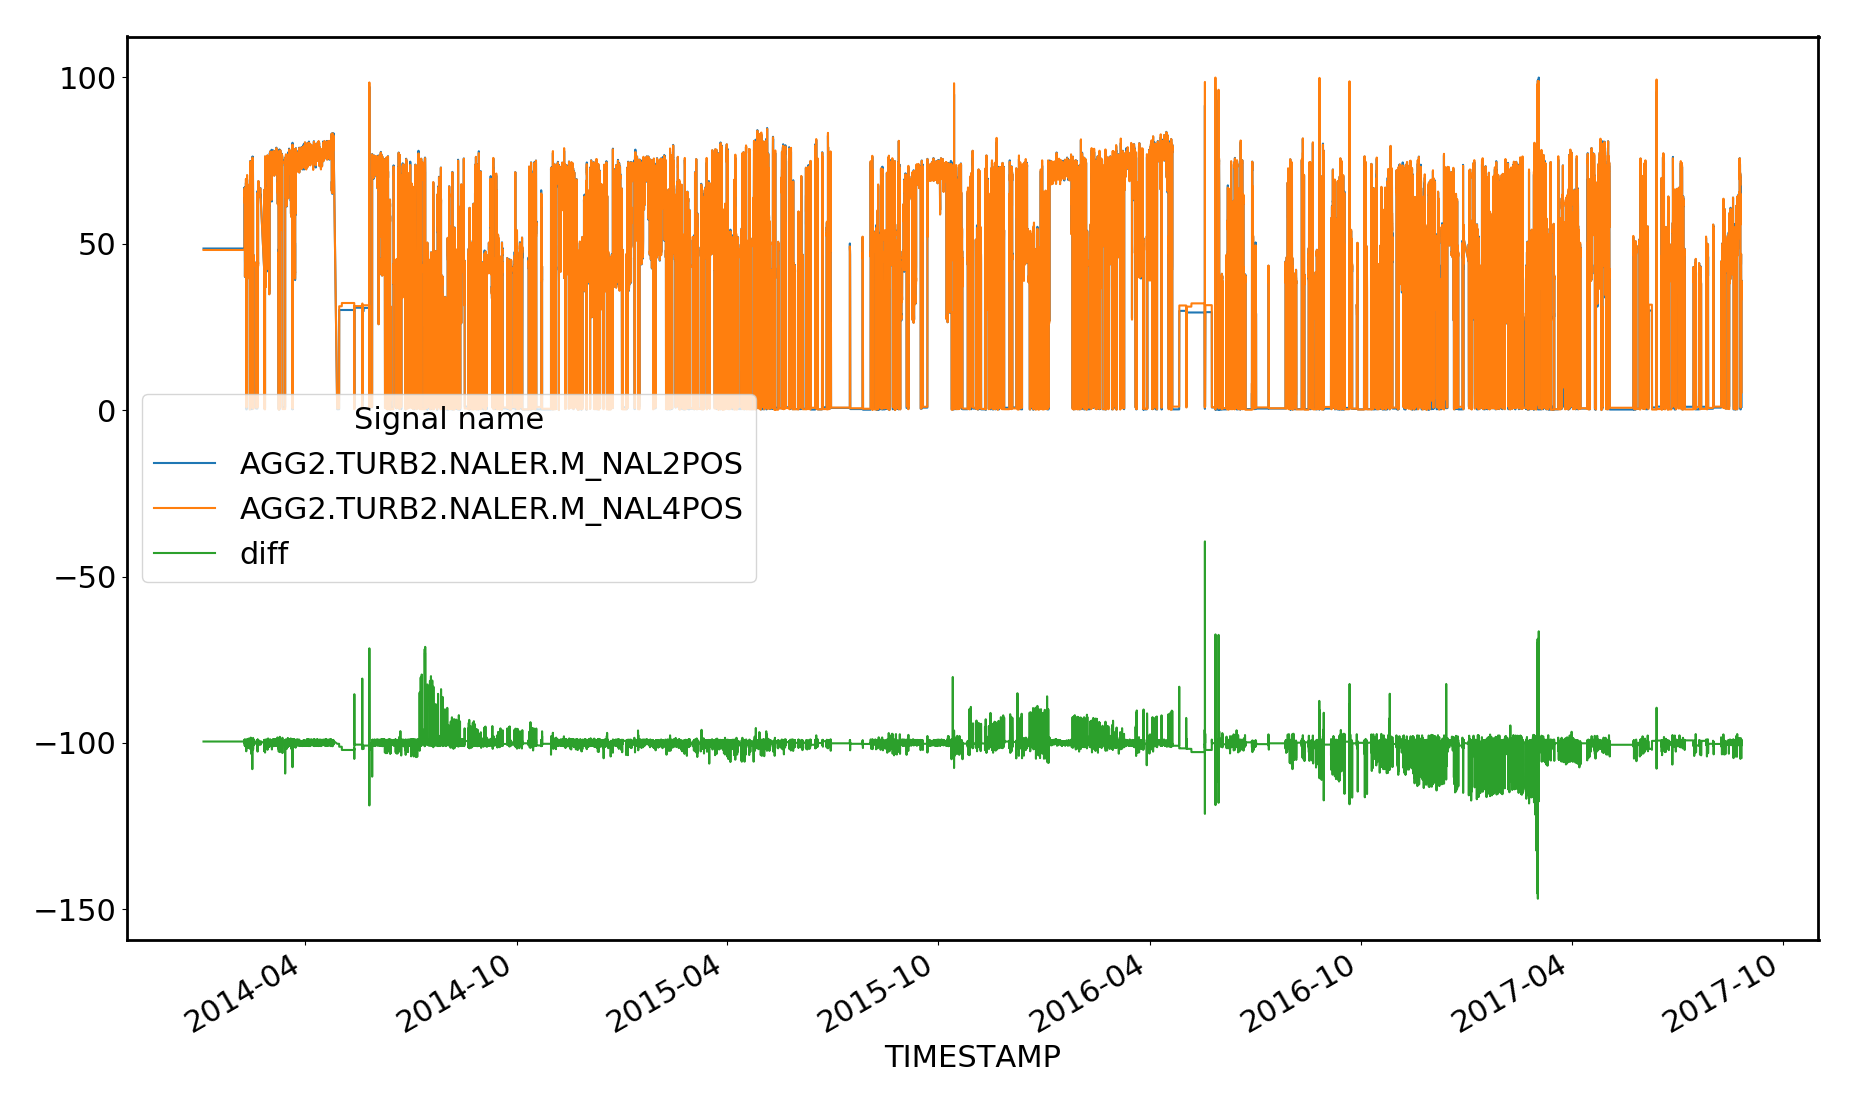
\includegraphics[width=\textwidth]{report/figures/data/turbine2_needle2_4.png}
            \caption{Needle 2 and 4 plotted on top of each other is seen in orange and blue at the top of the figure. With an offset of -100 the needle difference is seen in green. The dates are seen along the x-axis.}
            \label{fig:plant1_needle_error}
        \end{figure}
        
        
    \subsection{Other Pelton needle incidents}\label{subsec:start_failures}
        The log reported two other issues with the turbine needles at Plant $1$, that is observable in a scatter plot. This is seen in Figure \ref{fig:start_failure_turb1} and \ref{fig:start_failure_turb2}. Both are start-up failures due to problems with the needle operation.
        \begin{figure}[h!]
            % \caption*{Start up errors}
            \begin{minipage}[b]{0.49\linewidth}
                \centering
                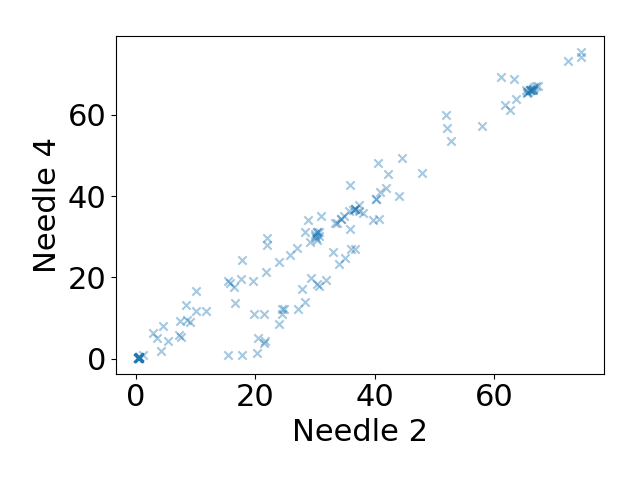
\includegraphics[width = \textwidth]{report/figures/data/turb1_n2_n4_scatter_start_failure_10122014.png}
                \caption{Turbine 1 start failure, 10.12.2014. Pairwise operated needles are scatterplotted against each other.}
                \label{fig:start_failure_turb1}
            \end{minipage}
            \hfill\vline\hfill
            \begin{minipage}[b]{0.49\linewidth}
                \centering
                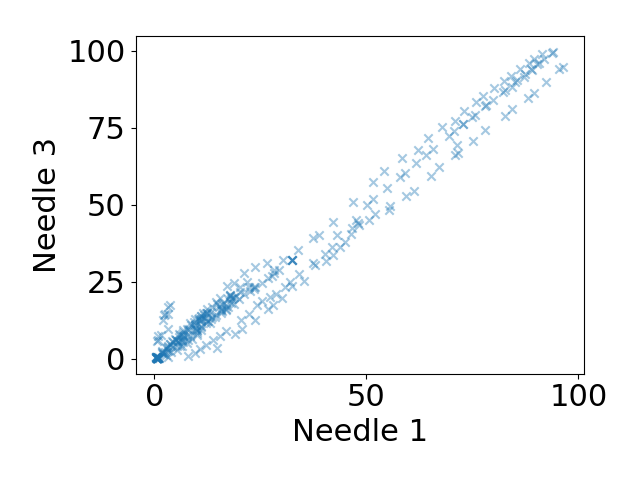
\includegraphics[width = \textwidth]{report/figures/data/turb2_n1_n3_start_failure_25082016.png}
                \caption{Turbine 2 start failure, 25.08.2016. Pairwise operated needles are scatterplotted against each other.}
                \label{fig:start_failure_turb2}
            \end{minipage}
        \end{figure}
        
        
    
    \subsection{Other plants with Pelton turbines}
        Further investigation showed that the second plant with Pelton turbines also has two turbines with pairwise operated needles. The third Pelton plant only has one turbine, and the needles are not pairwise operated. The turbine use from 1 to 5 needles depending on the produced power. Data from this plant could be used to generalize the anomaly detection methods to handle any combination of needles, but this will not be covered in this thesis. The needle operation for the second plant is seen in Figure \ref{fig:plant2_needles}. One can see that turbine $1$ has no sampling on needle $1$, but the three other pairs are sampled correctly. Plant 2 further motivates that there is something wrong with the needles for plant $1$. All needle pairs follow the linear pattern much better and have very few anomalies.
        \begin{figure}
            \begin{minipage}[b]{0.5\linewidth}
                \centering
                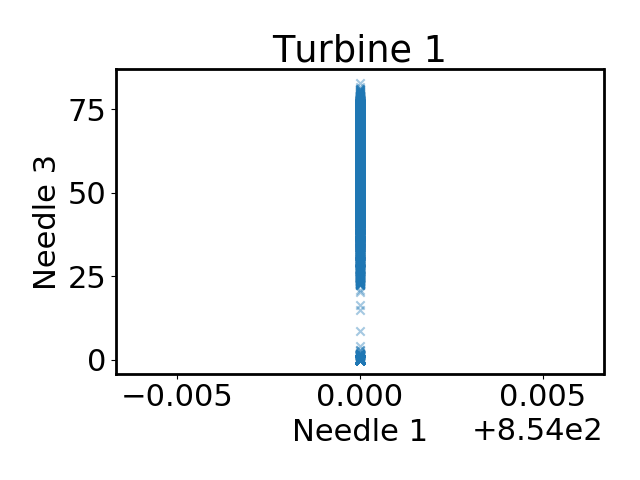
\includegraphics[width=\textwidth]{report/figures/data/p2_t1_n1_n3.png}
            \end{minipage}
            \begin{minipage}[b]{0.5\linewidth}
                \centering
                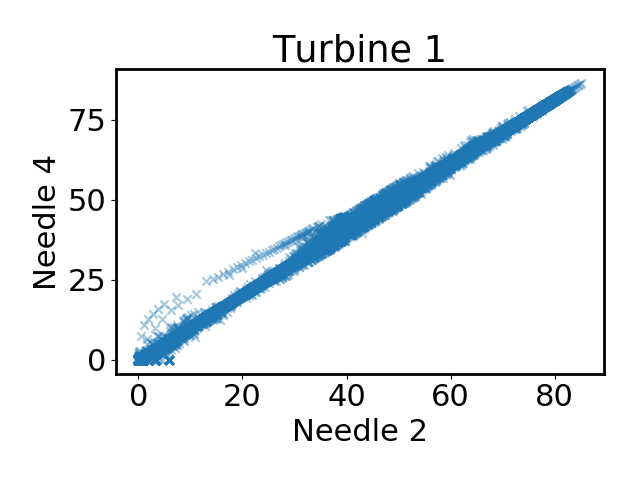
\includegraphics[width=\textwidth]{report/figures/data/p2_t1_n2_n4.png}
            \end{minipage}
            \begin{minipage}[b]{0.5\linewidth}
                \centering
                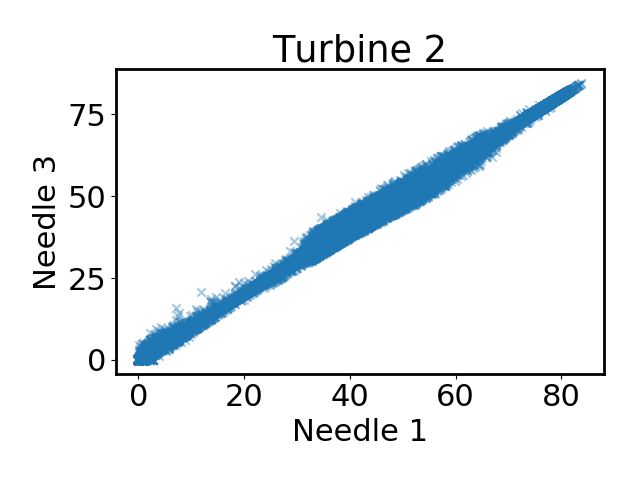
\includegraphics[width=\textwidth]{report/figures/data/p2_t2_n1_n3.png}
            \end{minipage}
            \begin{minipage}[b]{0.5\linewidth}
                \centering
                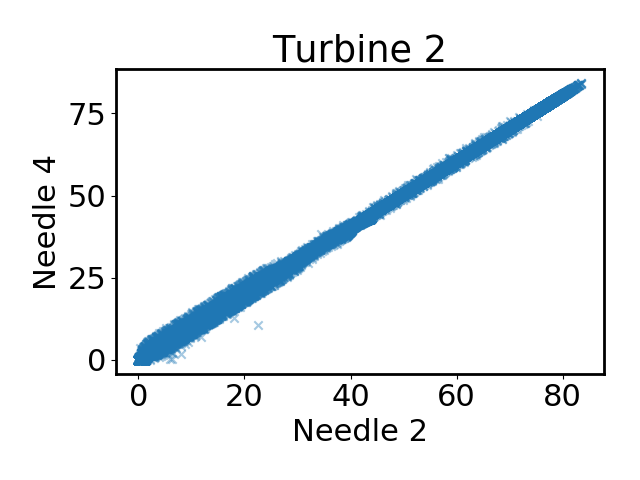
\includegraphics[width=\textwidth]{report/figures/data/p2_t2_n2_n4.png}
            \end{minipage}
            \caption{Needle openings for the pairwise operated needles for both turbines at Plant 2 are scatterplotted in four sub-figures.}
            \label{fig:plant2_needles}
        \end{figure}
        
        
        
    % \section{Other process signals}
        
    
        
    %     mention that this alone is a case one can build upon but track the error to other process-variable would be very interesting both for condition monitoring but also for identification of the fault and why it happened. 
        
        
    %     It is important to understand that an outlier in the data does not necessarily mean that something is about to break. There is a possibility that the sample is an indication of a condition change in the equipment, but it might also be due to an error in the measurement, noise or just a deviation in the ongoing process. This makes this kind of analysis even harder. An outlier might be coincident, that yields little to no information. 
        
         
         
    \subsection{Artificial case}\label{subsec:arti}
        Due to not having any incidents similar to the one seen at plant 1 turbine 2, an artificial error replicating the pattern is created. The primary motivation is to see when an error that is increasing over time is detectable. A subset of the data sampled at plant 2 is altered to replicate an error similar to the one seen for plant 1. By doing so, one knows exactly when the error starts occurring. This can then be used to evaluate how early different anomaly detection techniques detect anomalies.
    
        The turbine needles are controlled through a hydraulic system. A hydraulic system can suffer from many problems which can cause operational problems, such as pressure drops due to both external and internal leakage. External leakage is often broken hoses or pipes. Internal leakages are within the pumps and actuators. Both types of leakages reduce the system pressure and can slow down the motion of the system. Oil contamination can also be an issue if filters are not maintained at a given interval, unfiltered oil can then lead to clogged components, which can lead to pressure drops. The leading theory of the problems seen at plant 1 is that the oil flow is restricted in one direction. As needle 4 closes, the larger the differential pressure caused by the water head being restricted becomes. As the differential pressure grows, closing the needle requires more force. This means that if the hydraulic system is suffering from reduced capacity in one direction, the motion of the needle will slow down as the needle close. 
        
        Figure \ref{fig:plant2_arti_error} shows the colored scatter plot for the plant 2 data with and without the artificial error. As can be seen, it has a very similar pattern to what was seen at plant 1 in the days leading up to the reported incident. Figure \ref{fig:plant2_arti_error_40}, shows a close up on the lower openings of the needle. The deviation between the two needles increases with time, as seen in the case of plant 1. The artificial error is added to data sampled from needle pair [2,4] on turbine 2 at plant 2. Data from 20161001 to 20170401 is used, and the artificial error is added from 20170201.     
        
        \begin{figure}
            \begin{minipage}[b]{0.5\linewidth}
                \centering
                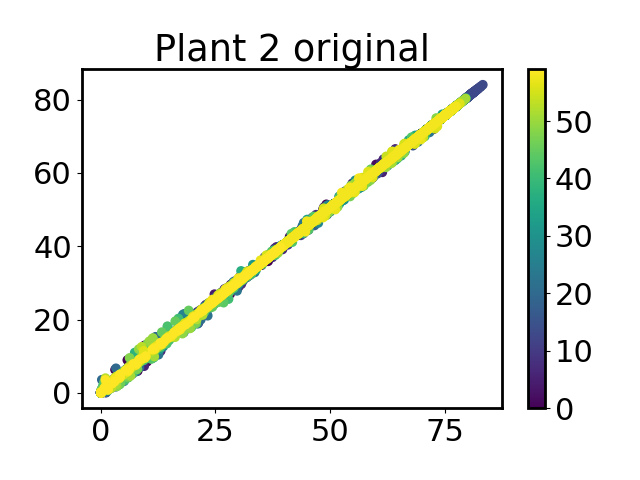
\includegraphics[width = \textwidth]{report/figures/analysis/artificial error/original_data_small.png}
                % \caption{Original data}
                % \label{fig:plant2_arti_orig}
            \end{minipage}
            \begin{minipage}[b]{0.5\linewidth}
                \centering
                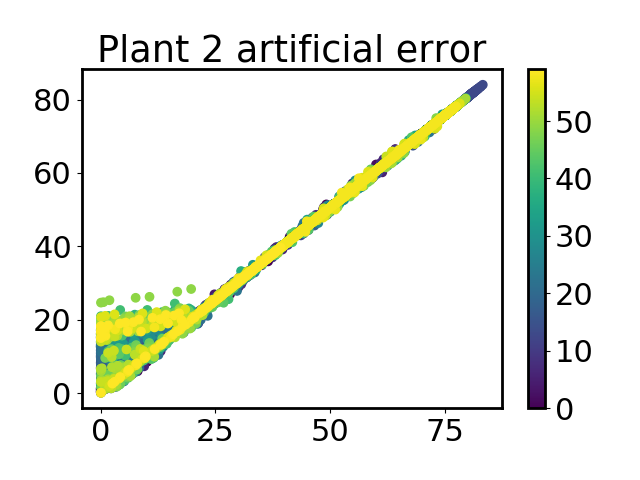
\includegraphics[width = \textwidth]{report/figures/analysis/artificial error/plant2_arti_error_small.png}
                % \caption{Added artificial error}
                % \label{fig:plant2_arti_error}
            \end{minipage}
            \caption{Colored scatter plot of the data before and after adding the artificial error. The original data is seen in to the left. How to interpret the figure can be found in Figure \ref{fig:plan1_scatter_20161001-20170304}.}
            \label{fig:plant2_arti_error}
        \end{figure}
        
        \begin{figure}
            \centering
            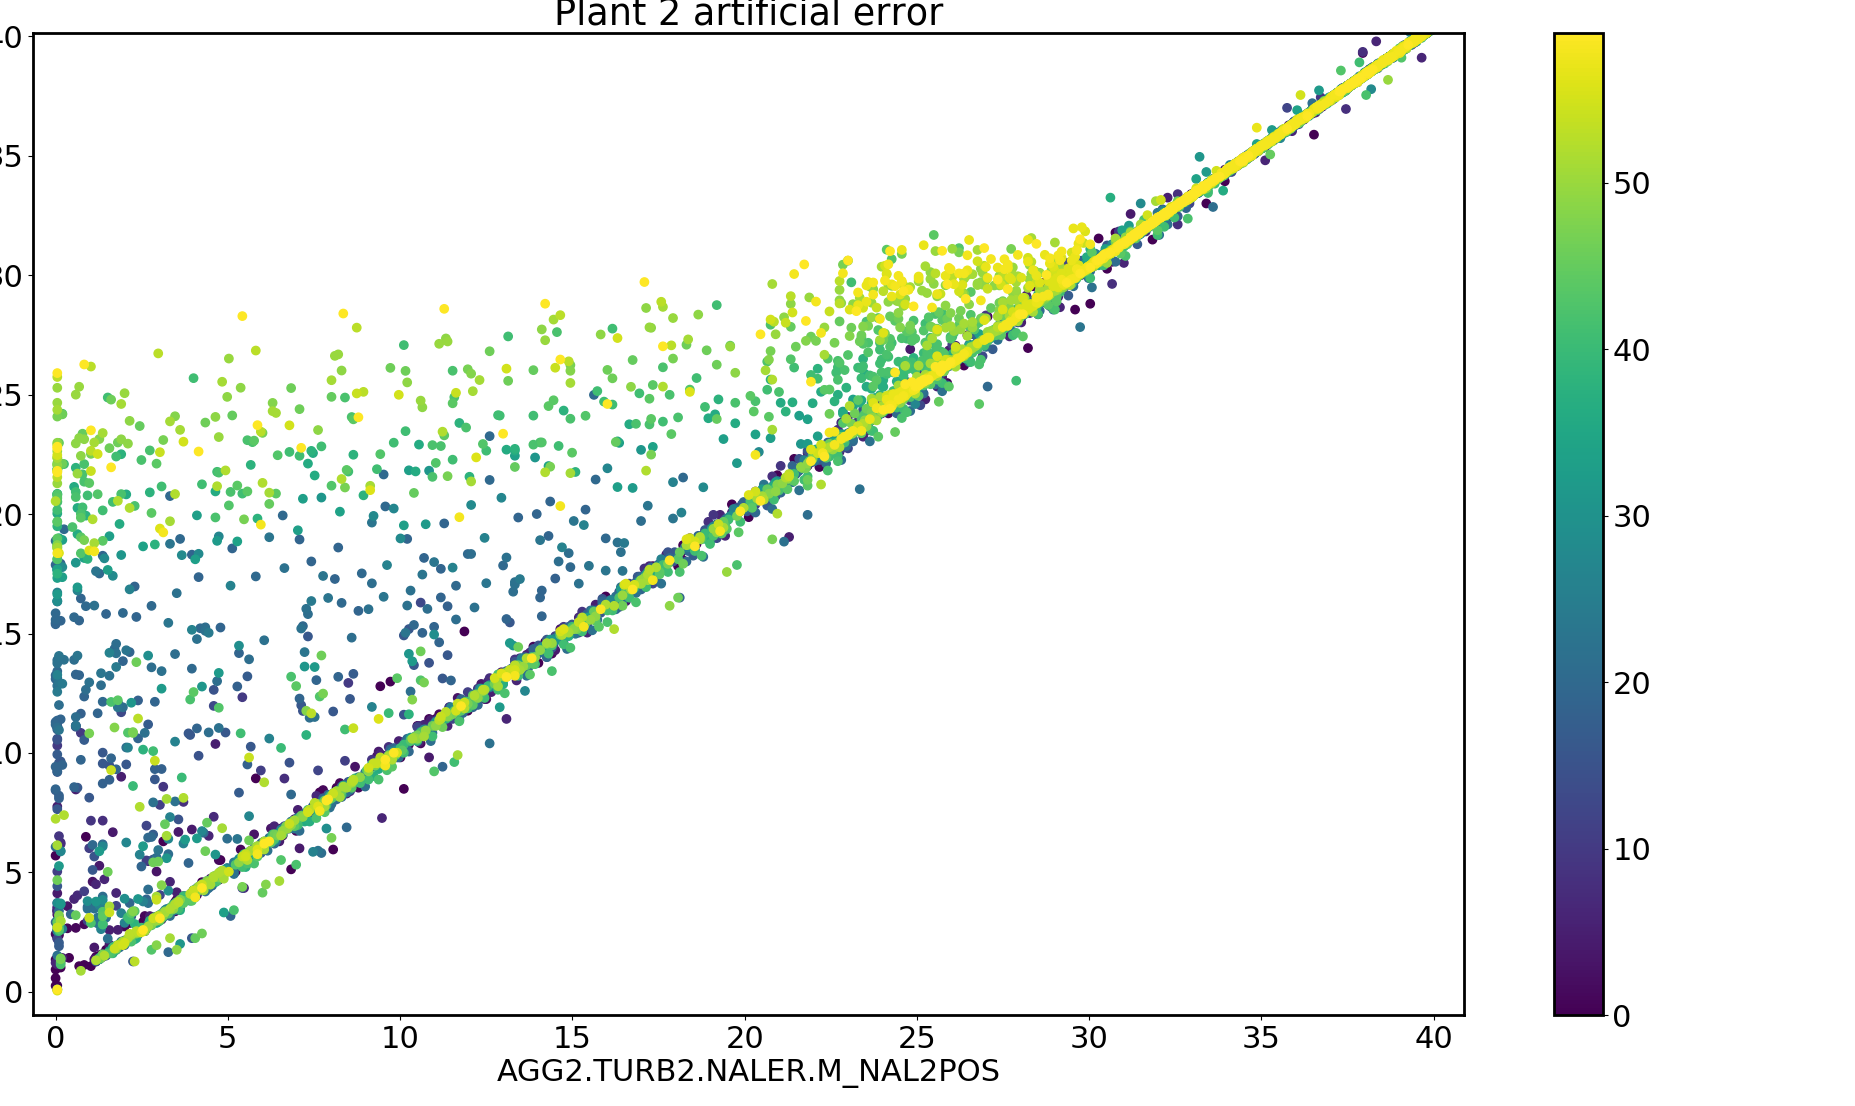
\includegraphics[width = \textwidth]{report/figures/analysis/artificial error/plant2_artificial_error_scatter_colored_40.png}
            \caption{Colored scatterplot of the artificial error for the lower openings. How to interpret the figure is found in Figure \ref{fig:plan1_scatter_20161001-20170304}.}
            \label{fig:plant2_arti_error_40}
        \end{figure}